\section{Client}

Zur Realisierung des Clients wird auf die etwas komforablere Scriptsprache CoffeeScript
zurückgegriffen. CoffeeScript-Code is gegenüber \acr{js}-Code deutlich kürzer, (Etwa 30\%) und hat
eine an Funktionale Sprachen wie Haskell erinnernde Syntax. Da mit den neuen Möglichkeiten in Play
2.1 CoffeeScript problemlos verwendet werden kann (Der Browser erhält kompiliertes \acr{js}) ,
entstehen hierdurch keine Nachteile.

Zur Strukturierung wird RequireJS sowie BackboneJS (und damit implizit auch UnderscoreJS) verwendet.
Durch die vielfältigen Möglichkeiten dieser Bibliotheken ist es möglich den Code klar zu
modularisieren.

\subsection{Browserkompatibilität}
\label{sec:comp}

Auf Grund der in \ref{sec:ws} beschriebenen Notwendigkeit, kann auf WebSockets nicht verzichtet
werden. Damit sind die meisten älteren Browser nicht mit der Anwendung kompatibel. 

\begin{table}[h]
\centering
\label{tab:comp}
\begin{tabular}{rlllll}
                  & \textbf{Chrome} & \textbf{Safari} & \textbf{IE} & \textbf{Firefox} 
                  & \textbf{Opera} \\\hline
  WebSockets      & 14.0            & 6.0             & 10.0        & 11.0             & 12.1  \\
  History API     & 5.0             & 5.0             & 10.0        & 4.0              & 11.5  \\
  WebWorkers      & 4.0             & 4.0             & 10.0        & 3.5              & 10.6  \\
  CSS Transitions & 4.0             & 3.1             & 10.0        & 4.0              & 10.5  \\

\end{tabular}
\caption{Kompatibilität der gängigsten Browser mit den Verwendeten Standards}
\captionsetup{font={footnotesize,bf,it}}
  \caption*{Datein von caniuse.com}
\end{table}

\TODO{Kompatibilitäts-Tabelle}

Aus Tabelle \ref{tab:comp} ist zu entnehmen, dass alle weiteren in der Anwendung benutzten Standards
eine geringere oder die gleiche Anforderung an die Aktualität des Browsers haben. Da WebSockets ein
sehr neues Konzept sind,  dienen sie als Orientierung: Alle Features, welche von jedem Browser, der
WebSockets unterstützt, auch unterstützt werden, dürfen verwendet werden. Alle anderen schließen wir
aus, da sonst die Zahl der potentiellen Nutzer weiter eingeschränkt würde. Die Anwendung ist damit
im Standardbrowser auf allen Systemen mit einem aktuellen Betriebssystem (Windows 8, Ubuntu 12.10,
OpenSUSE 12.2, OS X 10.8.2), sowie auf dem iPad, und aktuellen Windows RT Tablets benutzbar. Bei der
Entwicklung wurde jedoch besonderes Augenmerk auf WebKit-basierte Browser, insbesondere Google
Chrome gelegt und einige der anderen genannten Systeme sind ungetestet und damit ohne Gewähr.

\subsection{Benutzeroberfläche}

Bei der Gestaltung des \acr{ui} wurde besonderes Augenmerk auf die User Experience gelegt
um die Produktivität und die Zufriedenheit der Nutzer zu optimieren. \cite{emotionaldesign}
Inspiriert wurde das Design durch die von Microsoft in Windows Phone 7 bzw. Window 8 eingeführte
Design Sprache \textit{Metro UI} (bzw. seit 2012 \textit{Microsoft Design Language}). \cite{metroui}
Dabei wird auf unnötige Grafiken verzichtet und die Typographie in den Vordergrund gestellt. Durch
die Reduktion auf das Wesentliche entsteht eine neue Ästhetik welche eine willkommene Auffrischung
der Icon- und Fensterbasierten Oberflächen wie sie seit jeher bestehen, bietet.

\begin{figure}[ht]
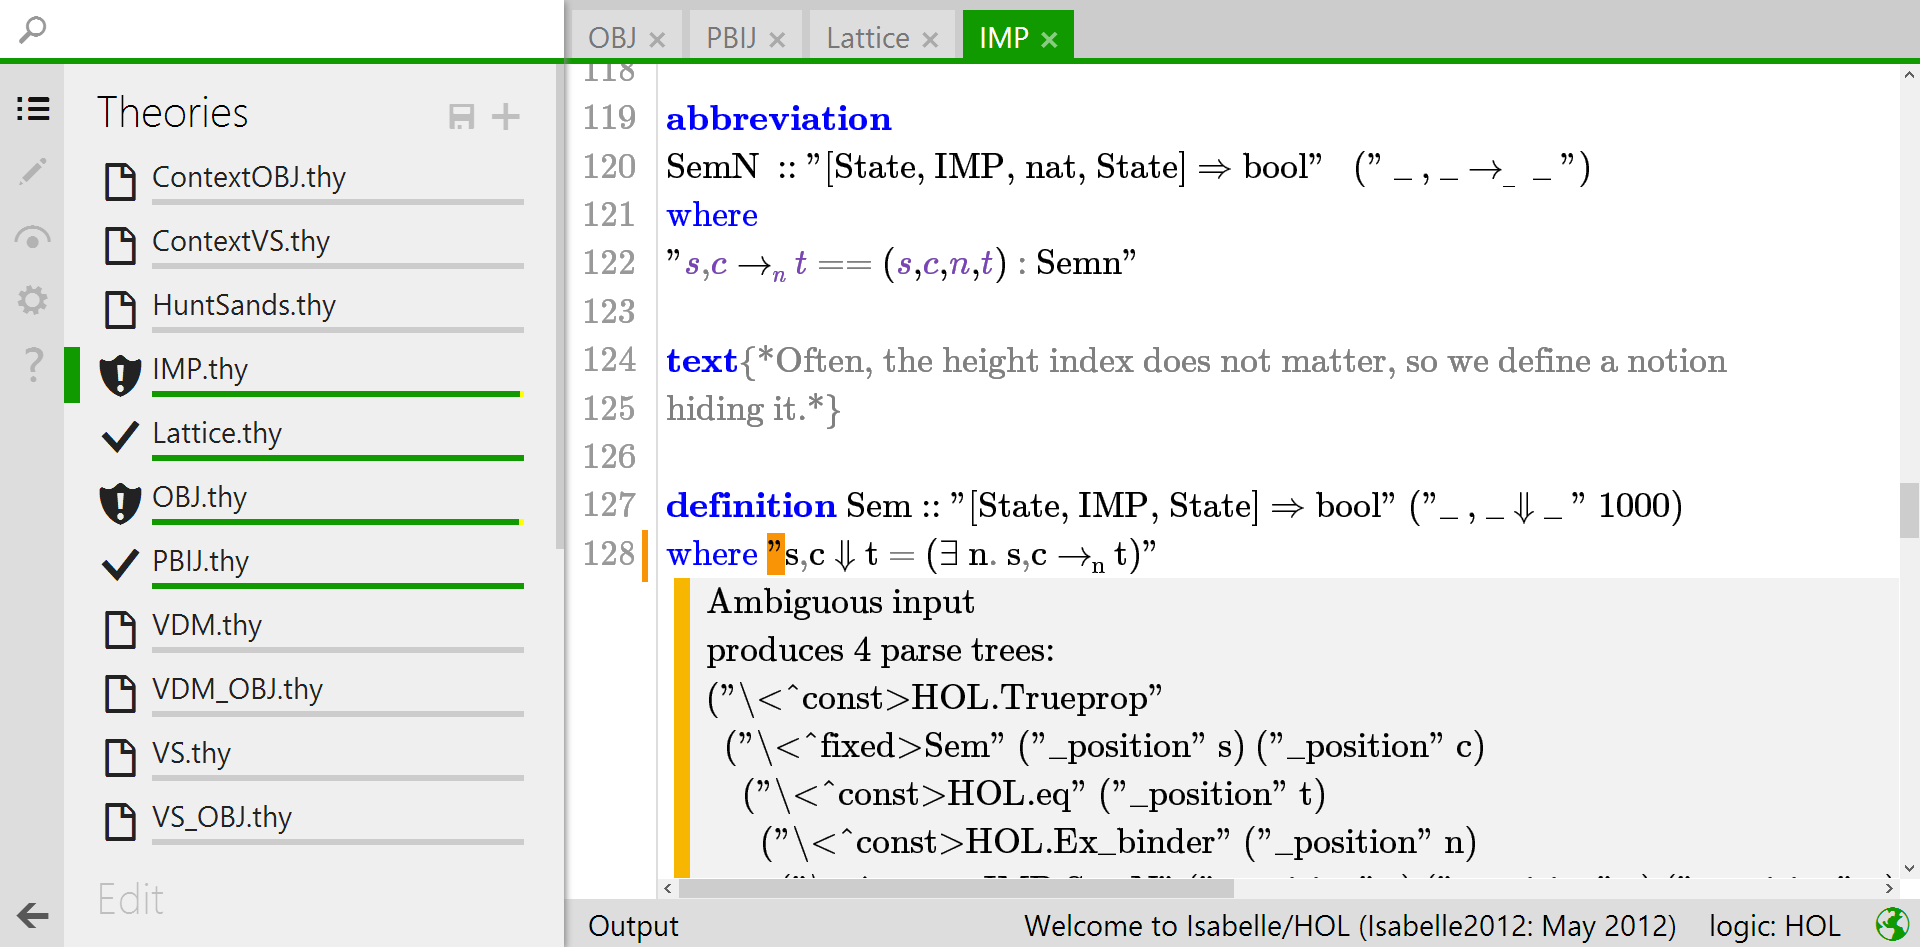
\includegraphics[width=\linewidth]{images/screen-main}
  \caption{Die clide-Oberfläche}
  \label{fig:screen-main}
\end{figure}

Besondere Herausforderungen sind das sinnvolle Unterbringen der Beweiszustände und
Fehlerinformationen in der Darstellung sowie die Darstellung des Fortschritts, der einzelnen
Theorien, welche nicht zwingend vom Nutzer geöffnet werden müssen sondern auch implizit als
Abhängigkeiten anderer Beweisdokumente verarbeitet werden können.

\subsubsection{Login}

Der Anmeldebildschirm (Login) ist entsprechend einfach gehalten. Dem Nutzer wird lediglich ein
Formular zur Eingabe von Benutzernamen und Passwort präsentiert. (Siehe Abbildung 
\ref{fig:screen-login})

Die Kommunikation erfolgt an dieser Stelle noch über normales \acr{http} und bei Fehlerhaften
Eingaben wird auf einer neu geladenen Seite eine Fehlermeldung über dem Formular angezeigt. Das
stört an dieser Stelle nicht und eine Nutzung von WebSockets würde die Sache hier nur
verkomplizieren, da so nicht die bereits ausgereiften Verfahren zur Anmeldung über \acr{http}
genutzt werden könnten.

\begin{figure}[ht]
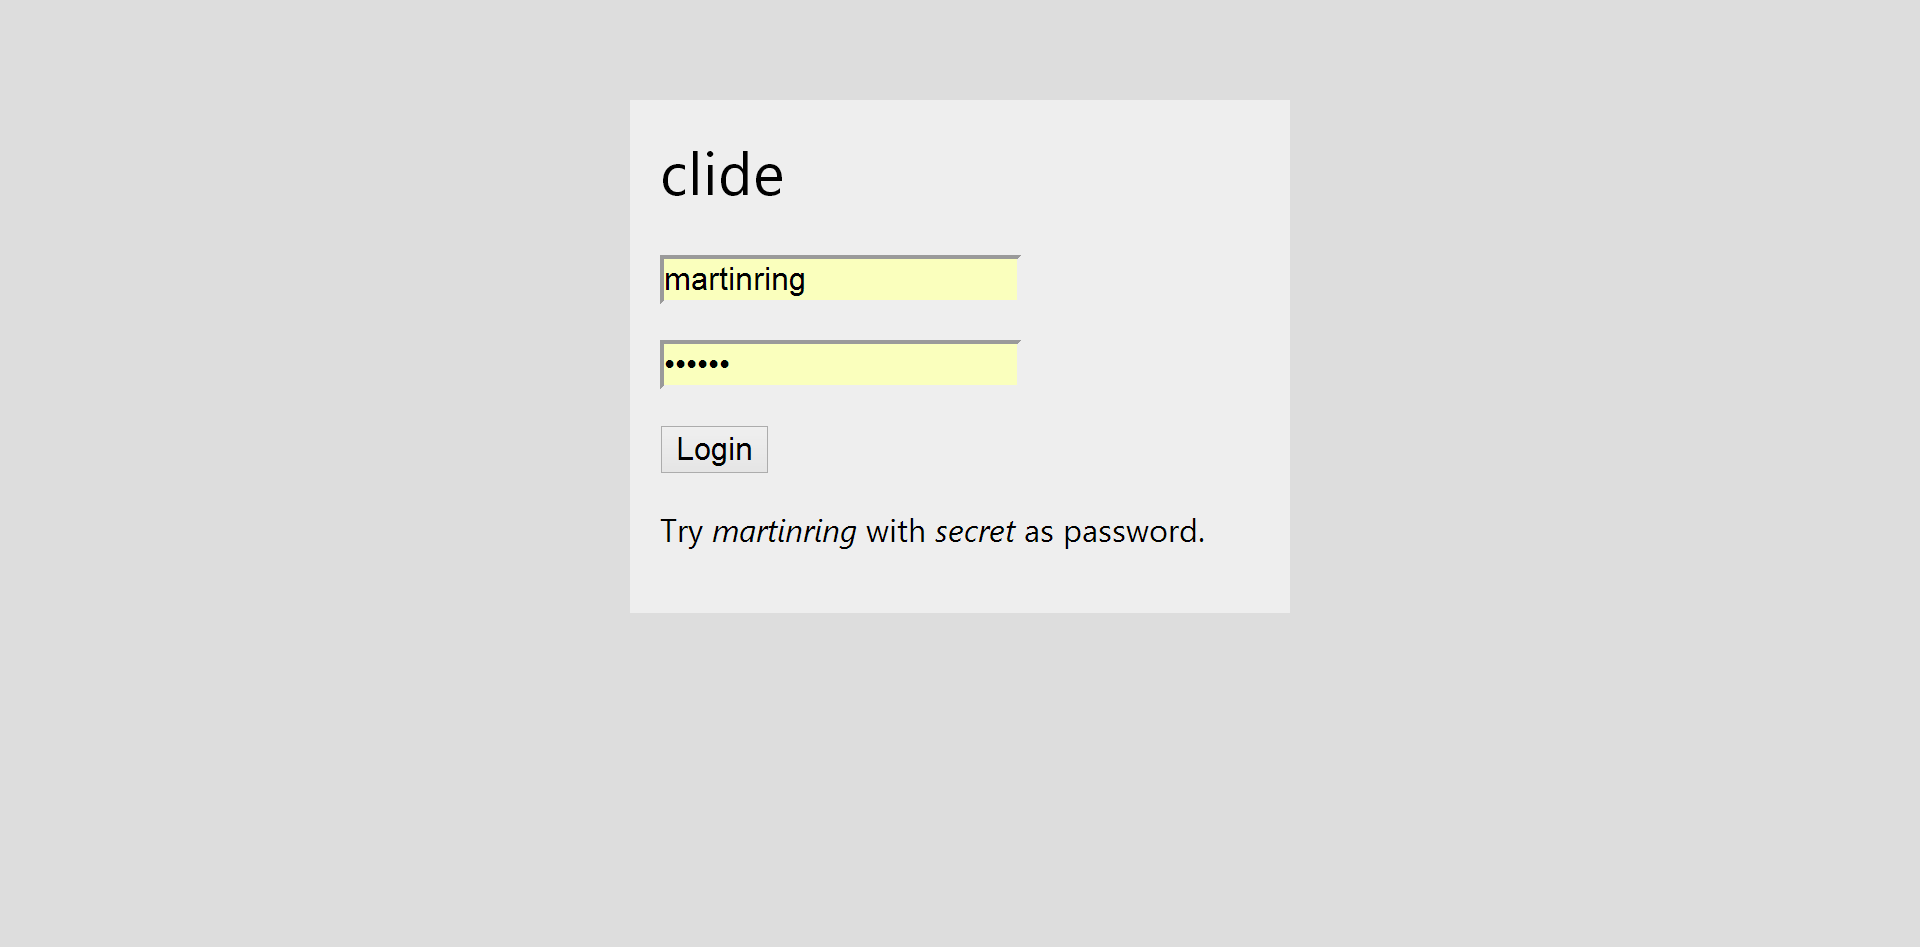
\includegraphics[width=\linewidth]{images/screen-login}
  \caption{Das Anmeldeformular}
  \label{fig:screen-login}
\end{figure}

\subsubsection{Projektübersicht}

\begin{figure}[ht]
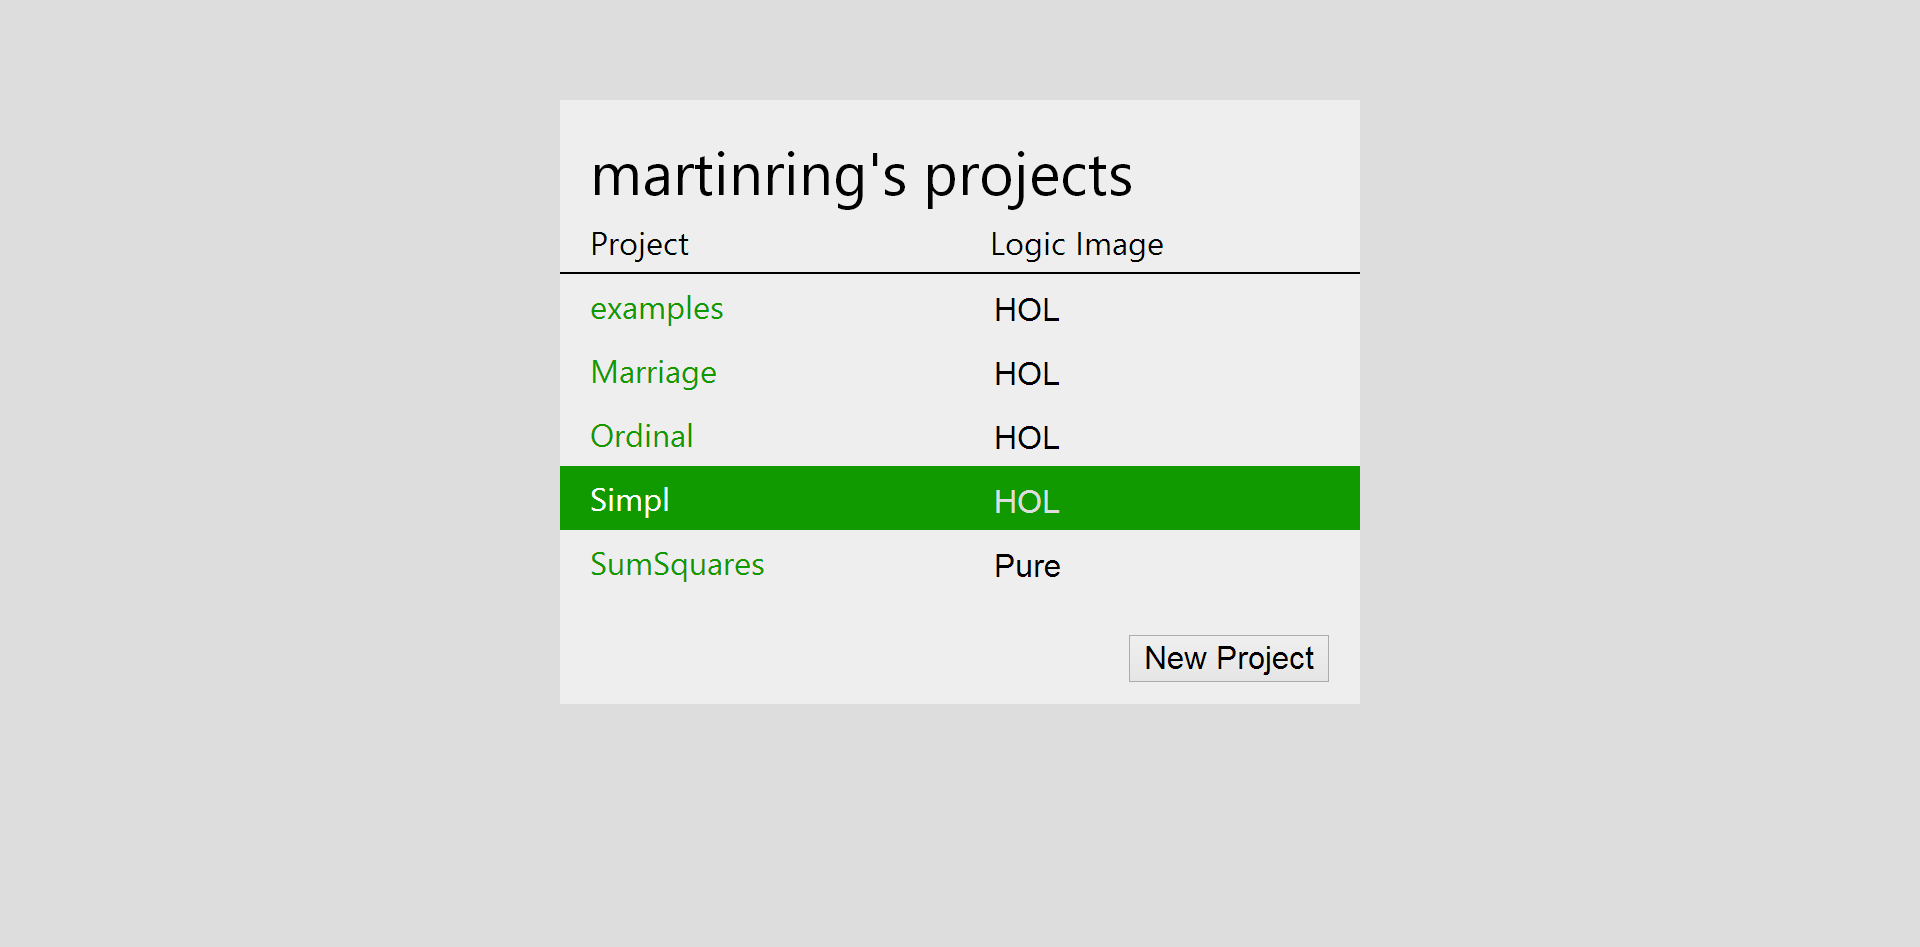
\includegraphics[width=\linewidth]{images/screen-projects}
  \caption{Die Projektübersicht}
  \label{fig:screen-projects}
\end{figure}

\subsubsection{Die Sidebar}

\begin{figure}[ht]
\centering
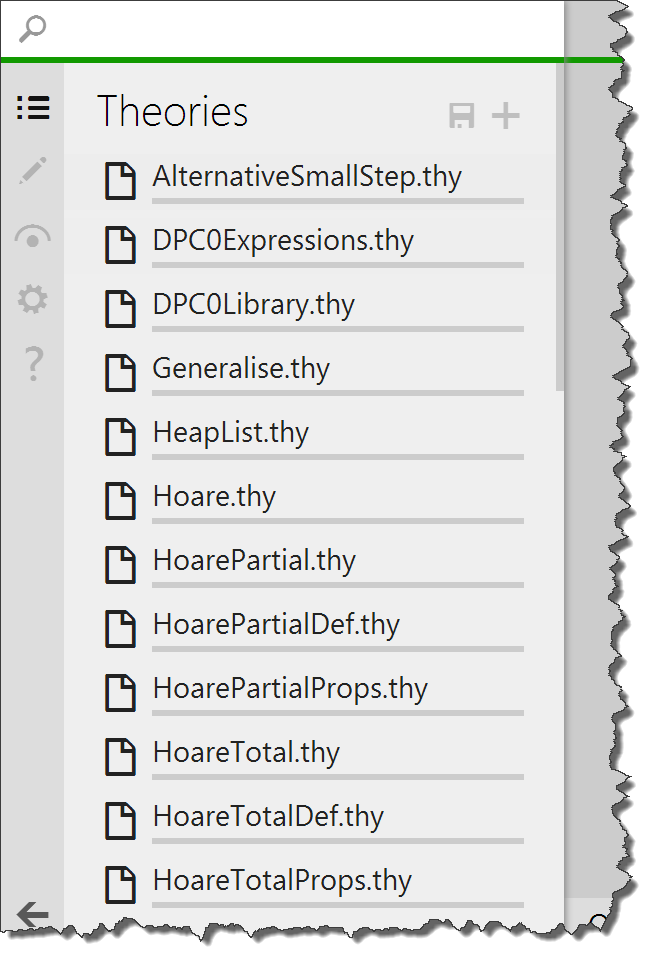
\includegraphics[width=0.4\linewidth]{images/screen-sidebar}
  \caption{Die Sidebar}
  \label{fig:screen-sidebar}
\end{figure}

\subsubsection{Webfonts}

\subsubsection{Die Editor-Komponente}
\label{sec:editor}

Die wichtigste Benutzerkomponente einer Entwicklungsumgebung ist der Text-Editor. Ein Editor für
Isabelle-Code hat hierbei besondere Anforderungen: Während in der Praxis bislang nur rudimentäre
Unterstützung für die Darstellung von Isabelle-Sonderzeichen und insbesondere von Sub- und
Superskript existierte, hat Isabelle/jEdit bereits eine stärkere Integration dieser eigentlich recht
essentiellen Visualisierungen eingeführt. \cite{iscala} Da bei der \acr{html}-Darstellung kaum
Grenzen gesetzt sind und sich \acr{css}-Formatierung sehr leicht dazu benutzen lässt bestimmte Text-
Inhalte besonders darzustellen, ist es klar, dass unsere Entwicklungsumgebung an dieser Stelle
besonders glänzen soll.

In einem ersten Prototypen war es möglich eine \acr{js}-Komponente zu entwickeln, welche es zuließ,
Isabelle-Code zu bearbeiten, sodass Sub- und Superskript sowie die Sonderzeichen korrekt dargestellt
wurden und bearbeitet werden konnten. Die besondere Anforderung bei ist hierbei nicht die
Darstellung sondern vor allem der Umgang mit den variablen Breiten. Selbst wenn ein Monospace-Font
verwendet würde, besteht das Problem, dass z.b. bei Sub- und Superskript nach Typographischen
Standards nur 66\% der Textgröße verwendet wird und somit auch die Zeichenbreite geringer wird. Da
aber eben die Visualisierung eine besondere Stärke der Anwendung sein soll, wollen wir zusätzlich
auch nicht darauf verzichten Ähnliche Fonts zu verwenden, wie in der Ausgabe der LaTeX-Dateien, also
auch Mathematische Sonderzeichen nicht in ein Raster quetschen. 

Eine weitere besondere Anforderung, welche bislang relativ einmalig zu sein scheint, ist die
Tatsache, dass das Syntax-Highlighting zu Teilen auf dem Server stattfinden soll und somit eine
Möglichkeit bestehen muss diese zusätzlichen Informationen in die Darstellung zu integrieren.

Zusammenfassend können folgende besondere Anforderungen an die Editor-Komponente formuliert werden:
Der Editor muss in der Lage sein

\begin{itemize}
  \item Syntaxhighlighting zu betreiben,
  \item Externes Syntaxhighlighting verzögert zu integrieren,
  \item Schriftarten mit variabler Zeichenbreite anzuzeigen,
  \item Tooltips für Typinformationen o.ä. anzuzeigen und
  \item Isabelle-Sonderzeichen zu substituieren.
\end{itemize}

Da der Hauptsächliche Aufwand bei einer Editor-Komponente nicht darin liegt Text zu bearbeiten und
darzustellen sondern vor allem in der Infrastruktur drumherum (Copy/Paste, Suche, Selektieren,
Drag'n'Drop, usw.) ist es verlockend, eine fertige Komponente zu verwenden. Hier existieren mehrere
ausgereifte Alternativen. Bei genauerer Betrachtung gibt es jedoch keine, welche optimal für unsere
Zwecke geeignet ist. 

\begin{description} 

\item {Der \textbf{MDK-Editor}\footnote{http://www.mdk-photo.com/Editor/}} bietet viele Features, wird
aber seit 2008 nicht mehr weiter entwickelt und scheidet damit sofort aus.

\item {Der \textbf{\acr{ace}}\footnote{http://ace.ajax.org/}} (Ehemals Mozilla SkyWriter) wird
momentan sehr stark weiter entwickelt. \acr{ace} bietet bereits ein ausgeklügeltes Framework für das
Syntaxhighlighting, welches sich in einem Prototyp relativ leicht an das Serverseitige
Syntaxhighlighting anbinden ließ. \acr{ace} bietet alle Funktionen, welche man von einem Modernen
Text-Editor erwartet, hat jedoch einen entscheidenden Nachteil: Zur Darstellung wird aus
Performance-Gründen intern ein festes Raster verwendet. Dabei wird davon ausgegangen, dass ein
Monospace Font verwendet wird. Von diesem wird einmalig eine Zeichenbreite ermittelt und diese feste
Metrik wird dann für alle internen Operationen verwendet. Da diese Designentscheidung so
tiefgreifend ist, scheint es nicht realistisch in akzeptabler Zeit, die Komponente so zu
modifizieren, dass variable Breiten unterstützt werden können. Außerdem ist es nicht möglich
Textstellen durch Sonderzeichen zu Substituieren. Somit scheidet auch \acr{ace} für die Verwendung
in der Anwendung aus.

\item {\textbf{CodeMirror}\footnote{http://codemirror.net/}} ist ebenfalls eine weit entwickelte
Editor-Komponente, welche nicht ganz so umfangreich, wie acr{ace} ist, jedoch um einiges flexibler
erscheint. In einem Prototyp war es möglich einige eigene Modifikationen für die Darstellung (Sub-
Superskript, Tooltips, Hyperlinks) zu integrieren. CodeMirror verwendet kein festes Raster, darunter
leidet die Performanz. Da wir jedoch darauf angwiesen sind, müssen wie diese Einbußen in der
Geschwindigkeit akzeptieren. Seit Version 3.0 welche am 10.12.2012 erschien, ist es möglich
Textteile zu durch HTML- Widgets zu substituieren. Dadurch ist es möglich Isabelle Sonderzeichen
welche durch ASCII Sequenzen wie beispielsweise \texttt{\textbackslash\textless
rightarrow\textgreater} für das Zeichen $\rightarrow$ repräsentiert werden direkt im Editor zu
ersetzen, sodass der bearbeitete Text valider Isabelle-Code bleibt, die Darstellung hingegen der
eines LaTeX-Dokuments entspricht.

\end{description}

Weitere Editoren existieren zwar, scheiden aber alle aus, da die meisten nicht einmal die Hälfte der
oben formulierten Anforderungen erfüllen. Es wird klar, dass CodeMirror der am besten geeignete
Editor ist. Trotzdem müssen einige eigene Anpassungen in den Kern des Editors integriert werden.
Diese sind unter anderem die Unterstützung von

\begin{itemize}
  \item Sub- und Superskript (sowie angepassten Cursorpositionen und -höhen),
  \item Tooltips für einzelne Textabschnitte sowie
  \item die Darstellung von Hyperlinks im Text.
\end{itemize}

\subsubsection{Beweiszustände}

\TODO{Beweiszustände}

\subsection{Modell auf dem Client}

Der Client muss zu jeder Zeit über ein konsistentes Abbild der relevanten Informationen verfügen.
Das stellt sich als schwierige Herausforderung heraus. Insbesondere müssen der Inhalt des
Texteditors mit dem Server synchron gehalten werden. Abbildung \ref{fig:diagram-workflow} zeigt ein
Vereinfachtes Abbild des Datenflusses in der Anwendung. Die besondere Schwierigkeit liegt darin,
dass natürlich nicht jeder Tastendruck übertragen werden kann. Das würde auch wenig Sinn machen, da
es nicht realistisch ist, jede einzelne Veränderung zu überprüfen. Den Nutzer würden Fehlermeldungen
zu Zwischenzuständen stören und der Server wäre absolut überlastet. Also wird nach jedem Tastendruck
ein \textit{Timeout} von 700 Millisekunden gestartet. Wenn es abläuft, ohne dass eine Taste gedrückt
wird, werden die Veränderungen im Dokument an den Server übertragen. In dem häufigen Fall eines
weiteren Tastendrucks innerhalb der Zeispanne, wird das Timeout neu gestartet (\textit{Reset}) so
lange, bis der Nutzer über den Zeitraum von 700ms keine Veränderung mehr vornimmt.

Die Zeitspanne von 700 Millisekunden hat sich in eigenen Experimenten als guter Wert herausgestellt
und ähnliche Werte werden auch von anderen Entwicklungsumgebungen und Editoren (\acr{ace}, eclipse,
Visual Studio, ...), Standardmäßig verwendet um den Präsentationskompiler zu entlasten.

\TODO{Client-Modell}